% Kompiliert mit pdfLaTex
%
% Institut für Operations Research
% Lehrstuhl für stochastische Optimierung
% Prof. dr. Steffen Rebennack
%
%%

\documentclass[a4paper,12pt]{article}

\usepackage[ansinew]{inputenc} % Bei Benutzung von Apple-Betriebssystemen bitte durch ``\usepackage[applemac]{inputenc}'' ersetzen.
\usepackage[T1]{fontenc}
 
\usepackage[english]{babel} 
%\usepackage[nospace,noadjust]{cite}
\usepackage{xcolor}
\usepackage{eurosym}
\usepackage{amssymb,amsmath}

% \usepackage{biblatex}
% \addbibresource{references.bib}

\usepackage{graphicx} 
\usepackage{tikz}
\usepackage{float}
\usetikzlibrary[trees]
\usepackage{color}
\definecolor{kit}{cmyk}{1,0,.6,0}

\usepackage{hyperref}
\hypersetup{pdftoolbar=true,
            pdfmenubar=true,
            pdfpagemode=UseOutlines,
            bookmarksnumbered=true,
            linktocpage=true,
            colorlinks=false,
            %backref, % Entkommentieren, um zu sehen, ob alle Literaturstellen im Text zitiert werden.
            colorlinks=false
            }

\newtheorem{definition}{Definition}[section]
\newtheorem{theorem}[definition]{Theorem}
\newtheorem{lemma}[definition]{Lemma}
\newtheorem{corollary}[definition]{Corollary}
\newtheorem{remark}[definition]{Remark}
\newtheorem{example}[definition]{Example}
\newtheorem{algorithm}[definition]{Algorithm}


\setlength{\parindent}{0pt}
\parskip1.5ex

\newcommand{\R}{\mathbb R} % Beispiel für die Definition eines eigenen Befehls
\begin{document}
\begin{titlepage}

\begin{figure}
\begin{minipage}{0.2\textwidth}

\includegraphics[scale=.6]{kit_logo_de_4c_positiv-rgb.pdf}
\end{minipage}
\hfill
\begin{minipage}{0.6\textwidth}
\begin{flushright}
Institut f\"ur Operations Research \\
Lehrstuhl f\"ur stochastische Optimierung \\
Prof. Dr. Steffen Rebennack \\
\medskip
\end{flushright}
\end{minipage}
\bigskip
\end{figure}

\vspace*{35pt}

\begin{center}
\Large{Seminar}    

\vspace*{35pt}

\fboxsep 40pt
\fboxrule 6pt
\fcolorbox{kit}{white}{\parbox{80mm}{\begin{center}\Large{Neural Stochastic Dual Dynamic Programming}\\ \end{center}}}

\vspace*{40pt}

\normalsize

by \\[4ex]

Janik K\"onigshofer \\
Matr. Nr.: -------\\
Study program: Master\\[4ex]

Date\\
June 27, 2022 \\[4ex]

Adviser: Dr. John Alasdair Warwicker

\end{center}

\end{titlepage}
\thispagestyle{empty}\cleardoublepage

\mbox{}\thispagestyle{empty}\cleardoublepage

\vspace*{2eM}

{\Large \textbf{Erkl\"arung}} 
% Bitte prüfen Sie, ob dies die für Ihren Studiengang verlangte Erklärung ist!

\bigskip
Ich versichere wahrheitsgem\"a\ss, die Arbeit selbstst\"andig angefertigt und alle benutzten Hilfsmittel und Quellen vollst\"andig angegeben zu haben, die w\"ortlich oder inhaltlich \"ubernommenen Stellen als solche kenntlich gemacht zu haben und die Satzung des KIT zur Sicherung guter wissenschaftlicher Praxis beachtet zu haben.\\

\vspace*{3eM}

\textit{17.06.2022} \hspace{8cm} \textit{Janik K\"onigshofer}
\thispagestyle{empty}\cleardoublepage

\mbox{}\thispagestyle{empty}\cleardoublepage

\setcounter{page}{3}

\begin{abstract}
In practical applications, optimization problems often involve uncertainties. In order to handle these uncertainties, methods from stochastic optimization are needed. Unfortunately, these methods are often limited to low-dimensional problems, since they do not scale well for large problems, caused by the curse of dimensionality. 
One of the most commonly used approaches is the stochastic dual dynamic programming algorithm (SDDP), which has a worst-case complexity that scales exponential in the number of decision variables.
In this paper the approach of Neural Stochastic Dual Dynamic Programming by Dai and Xue et al. is discussed, an approach which augments SDDP, by utilizing neural networks in order to compute initial optimality cuts for a warm start of the SDDP algorithm and projecting the problem to a low-dimensional representation, to avoid the exponential increase in necessary iterations.
A possible real-world application of the NSDDP approach on the unit-commitment problem from Optimal Power Flow is presented and discussed. Own computations on a two-stage news-vendor problem illustrate the potential of the approach and highlight its advantages and disadvantages.
\end{abstract}
\thispagestyle{empty}\cleardoublepage

\mbox{}\thispagestyle{empty}\cleardoublepage

\tableofcontents

\newpage
\ \newpage

\section{Introduction} \label{Introdcution}
Optimization problems can be found in a variety of fields and have multiple applications, for instance in the energy sector \cite{PereiraPinto1991}, logistics, machine learning and many more.
In several industrial settings, the problem is decomposed into multiple stages.
% These stages are usually determined by the  like multiple time periods
These stages are usually defined in terms of time, but are not bound to a specific number of days or hours. For example, a problem that lasts for more than a year, can still be decomposed into two stages if the problem structure only changes once.
These problems arise in a multitude of settings like fleet management \cite{example_powell_fleet_management}, supply-chain optimization \cite{example_supply_chain_optimization}, portfolio optimization \cite{example_portfolio_opt} and power scheduling in a Hydro-Thermal System \cite{example_power_scheduling_Nowak2000}.
These problems involve making decisions based on current knowledge.
After the execution of the first-stage decision, new information from the environment is observed and is used for a successive decision.
Optimization problems from this kind of problem class are called sequential decision problems \cite{Powell_solving_Curses_of_Dimensionality}.\\
% The problem class of these kind of optimization problems are called sequential decision problems \cite{Powell_solving_Curses_of_Dimensionality}.\\
Since these sequential decision problems are calculating decisions over a time frame,
it would be a strong assumption to consider them deterministic, hence they are assumed as stochastic.
One approach to solving optimization problems under uncertainty is stochastic optimization.
According to Powell \cite{POWELL2019795,Powell_Clearing_the_Jungle_of_stochastic_Optimization}, stochastic optimization has many research streams, the major ones being stochastic dynamic optimization and stochastic programming.
Stochastic programming is more common in operations research fields, while stochastic dynamic programming is used in optimal control, like in electrical engineering.
Both frameworks will be briefly discussed in this seminar paper.

This paper discusses the new advances made in the paper 'Neural Stochastic Dual Dynamic Programming' by Dai and Xue et al. \cite{NSDDP}.\\
First, a quick introduction is given to describe different frameworks in order to solve sequential optimization problems, namely stochastic programming and stochastic dynamic programming.
After that, a short overview of the major challenges of these methods is presented, namely the curse of dimensionality.
In the next section, the current state-of-the-art approaches out of the framework of stochastic programming for solving these problems are
presented, namely the L-shaped method, an extension of Benders decomposition, and stochastic dual dynamic programming.
For each approach, the pros and cons are discussed.
Moreover, the neural stochastic dual programming approach from Dai and Xue et al. \cite{NSDDP} is presented in detail with an emphasis on the advantages and disadvantages over current solving methods, and also what the limitations and constraints of this approach are.
Following that section, own computations based on my implementation of the neural stochastic dual dynamic programming approach are presented.
Finally, a conclusion and an outlook on possible future research is given.

\subsection{Stochastic Optimization}
In the following section, the frameworks of stochastic programming and stochastic dynamic optimization are discussed.
They are similar in that they both try to find an optimal policy instead of finding an optimal solution.
An optimal policy is a function that provides an optimal solution given the current known information about the environment \cite{POWELL2019795}. 
The disparities and similarities of these two approaches will be discussed in the following sections.
\subsubsection{Stochastic Programming}\label{Stochastic Programming}
Stochastic programming is a framework from the field of operations research, which deals specifically with the solution of optimization problems that span over multiple periods and involve uncertainty. \\
Stochastic optimization problems, also often referred to in the literature as \glqq Stochastic Program\grqq{} or simply SP, are according to \cite{BirgeLouveaux} optimization problems where part of the information about the problem is uncertain. \\
A common approach to solve this class of problems is to split these problems into two time-discrete stages.
In the first stage, the problem is considered without the knowledge of the uncertain data in the future and is hence deterministic. However, the decision in the first stage, usually denoted by $x$, tries to hedge against future outcomes or possibly occurring future costs, by accounting for these in the objective function. \\
One method to do that is to measure the uncertainty of these stochastic future outcomes with an uncertainty measure \cite{Fuellner_SDDP_TUT}. 
The uncertainty measure of choice is usually the expectation, however other measures are also possible. For a detailed discussion of these measures, see \cite{BirgeLouveaux}.

After the first-stage decision is taken, new information $\omega$ from the environment is observed as a realization of a random variable $\xi$ that represents the stochastic process, where $\omega \in \Omega$ and $\Omega$ is the set of all possible outcomes. \\
That additional information can be used to derive a subsequent second-stage decision as a recourse, usually denoted by $y$ to account for the changes in the environment by which the first stage decision $x$ is no longer optimal. \cite{Fuellner_SDDP_TUT, BirgeLouveaux}.
Since $y$ is dependent on the realization $\omega$, the second stage decision is sometimes denoted as $y(\omega)$.

According to \cite{Lectures_on_stochastic_Programming_Shapiro_Ruszczynski}, the linear case of the described two-stage stochastic optimization problem can be formulated as follows
\begin{subequations}\label{stochastischeFormulierung}
    \begin{alignat}{3}
          &\min_x        &\quad& c^T x + \mathbb{E}_\xi \left[ Q(x,\xi(\omega))  \right] \label{SP_Zielfunktion mit EW}\\
          &\textrm{ s.t.}  &\quad& A x = b \\
          &              &\quad&x\geq0,
    \end{alignat}
\end{subequations}
where the function $Q$ is called the value function of the second stage and according to \cite{Lectures_on_stochastic_Programming_Shapiro_Ruszczynski} is given as
\begin{subequations}\label{Zweite_Stufe_Problem}
    \begin{alignat}{4}
         Q(x,\xi(\omega)) := & \min_y        &\quad& q^T(\omega)y  \\
                             & \textrm{ s.t.}  &\quad&W(\omega)y = h(\omega) - T(\omega)x \label{Recourse Gleichung}\\
                             &                &\quad&y\geq0.
    \end{alignat}
\end{subequations}
In most cases, the underlying stochastic process is represented as a scenario tree, where a sequence of realizations $\{\xi_t\}_{t=1}^{T}$ is called a scenario. \\
An example of a scenario tree for a problem with three stages and three possible stochastic outcomes at the first stage and two possible scenarios at the second stage is shown in figure \ref{fig:scenario_tree}.
This scenario tree has six different scenarios, one possible scenario, marked as \textit{scenario 6}, is highlighted in black.  \\
% Set the overall layout of the tree
\tikzstyle{level 1}=[level distance=3.5cm, sibling distance=3.5cm]
\tikzstyle{level 2}=[level distance=3.5cm, sibling distance=2cm]

% Define styles for bags and leafs
\tikzstyle{end} = [minimum width=3pt]
\tikzstyle{standard} = [circle,draw, minimum width=8pt,fill=gray]
\tikzstyle{scenario} = [circle,draw, minimum width=8pt,fill=black]
\begin{figure}[h]
    \centering
    \begin{tikzpicture}[grow=right, sloped, scale=0.7]
    \node[scenario] {}
        child [black] {
            node[scenario] {} % This is the first of three "Bag 2"
            child {
                node[scenario] {}
                child {
                    node[end] {Scenario 6}
                }
            }
            child [black] {node[standard] {}}
        }
        child [black] {
            node[scenario] {}
            child {
                node [scenario] {}
                    child {
                        node [end] {Scenario 3}
                    }
            }
            child {
                    node[standard] {}
            }
        }
        child [black] {
            node [scenario] {}
                child {% Here are three children, hence three end branches
                    node [standard] {}
                }
                child {
                    node [scenario] {}
                    child {
                        node [end] {Scenario 1}
                    }
                }
        }
    ;
    \end{tikzpicture}
    \caption{Scenario tree with two stages and six scenarios, inspired by \cite{Fuellner_SDDP_TUT, Powell_Clearing_the_Jungle_of_stochastic_Optimization}}
    \label{fig:scenario_tree}
\end{figure}
According to Powell \cite{Powell_solving_Curses_of_Dimensionality}, the sequence of decisions and events can then be stated as follows:
\begin{align*}
    x \rightarrow \xi(\omega) \rightarrow y(\omega,x) .
\end{align*}
The classical formulation of a stochastic optimization problem with recourse assumes a linear objective function, although extensions to the nonlinear case are also possible \cite{BirgeLouveaux}.
The principle of two-stage optimization can be easily transferred to the multistage case, but it introduces additional complexity. \\
According to \cite{Lectures_on_stochastic_Programming_Shapiro_Ruszczynski}, the multistage problem can be formulated as follows.

Let $\xi_t$ be a known random vector with a corresponding population $\Omega_t$ for the stage $t = 2, \dots,T$. $\Omega_t|\omega_{t-1}$ is the conditional population for the stage $t$, given that in stage $t-1$ the event $\omega_{t-1} \in \Omega_{t-1}$ has occurred. \\
A multistage optimization problem with time horizon $T > 2$ has the following structure, again restricting ourselves to the linear case:
\begin{subequations}\label{stochastische Multistage Formulierung}
    \begin{alignat}{2}
         \underset{x}{\min}  & \quad  c_1^T x_1  + \mathbb{E}_{\xi_2} [  \min c_2(\omega_2)x_2(\omega_2) + \mathbb{E}_{\xi_3}[\dots +                                                                                                 \mathbb{E}_{\xi_T}[ \min c_T(\omega_T)x_T(\omega_T)] ]  ]\\
      \textrm{s.t.}  & \quad W_1 x_1 = h_1                                                             \\
                     & \quad T_1 (\omega_2) x_1 + W_2 (\omega_2) x_2(\omega) =h_2(\omega_2),  \quad  \forall \omega_2 \in \Omega_2\\
                     & \quad \quad \vdots                                                                          \\
                      \begin{split}
                        \quad T_{T-1} (\omega_T) x_{T-1} + W_T (\omega_T) x_T(\omega)=h_T (\omega_T),   \\ 
                        \forall \omega_{T-1} \in      \Omega_{T-1},\, \omega_T \in \Omega_T \mid \omega_{T-1} 
                       \end{split} \\
                     &\quad x_1 , x_t(\omega_t) \geq 0                                                \quad   t= 2,\dots,T
    \end{alignat}
\end{subequations}
Problem \ref{stochastische Multistage Formulierung} is also called the extensive form of a stochastic program.
This is in fact the deterministic equivalent of the stochastic program, since for every possible scenario, an extra constraint is added to the problem \cite{BirgeLouveaux}.\\
This is a linear problem that can be solved by conventional solvers for LPs.
However, since the problem size can drastically increase if more complexities are added, large-scale optimization methods should be considered to solve this problem in reasonable computing time. \\
A further constraint is that the number of variables and constraints grow exponentially with an increasing number of stages.
Furthermore, this problem can only be solved for a discrete probability distribution, otherwise the problem has to be discretized, since problem \ref{stochastische Multistage Formulierung} would have an infinite number of constraints \cite{SDDP_Solver_Paper}.

 \subsubsection{Stochastic dynamic optimization} \label{stochastic_dynamic_programming}
Another research stream that focuses on solving multistage stochastic optimization problem is stochastic dynamic optimization.
This research stream is more focused on representing dynamic behavior in an optimization problem and on solving sequential decision problems by solving the well-known Bellman-Equation, which was first introduced by Bellman in 1957 \cite{Bellman1957}. \\
As before, the goal in this framework is not find a single optimal solution vector, but to find an optimal function or policy, that provides an optimal solution given an environmental state $S_t$ at time $t$.
According to Powell \cite{Powell_solving_Curses_of_Dimensionality}, this state describes all information that is necessary to make an optimal decision and is known at stage $t$.
The problem of finding this optimal policy can be traced back to solving the Bellman equation, according to \cite{Einfuehrung_in_das_OR}.
In e.g. \cite{Einfuehrung_in_das_OR} it has already been shown that the determination of an optimal policy or strategy and the optimal value of the problem can be traced back to the solution of the Bellman equation.
This equation has, according to \cite{Powell_solving_Curses_of_Dimensionality}, the form shown in equation \ref{Bellman-Gleichung} and provides an optimality condition for the value functions,
\begin{align}\label{Bellman-Gleichung}
       V_{t}(S_{t})& = \underset{x_{t}\in{\mathcal{X}_{t}}}{\min}\, C_{t}(S_{t},x_{t}) + \gamma \mathbb{E}\left[ V_t(S_{t+1}) \mid S_t \right]
\end{align}
with $V_t(S_t)$ being the value functions, describing the value of a state $S_t$ at a time $t$, provided an optimal strategy is followed from time $t$ \cite{Einfuehrung_in_das_OR}.
The term $C_{t}(S_{t},x_{t})$ represents a cost function that depends on the stage of the system $S_t$ and the chosen decision $x_t$, which is selected from the feasible set $\mathcal{X}_t$ of stage $t$.
The $\gamma$ represents a discount factor which describes how much the future outcomes are affecting present decisions \cite{Einfuehrung_in_das_OR, Powell_solving_Curses_of_Dimensionality}.
The discount factor can also be interpreted as a measure about how much the forecasts about the future outcomes are trusted. \\
After a decision $x_t$ is chosen and a realization from the underlying stochastic process can be observed, the environment transitions to the state $S_{t+1}$.
That state is determined by a transition function $S^M(S_t, x_t, \xi(\omega_t))$ \cite{Powell_solving_Curses_of_Dimensionality}.

Equation \ref{Bellman-Gleichung} shows that the multistage problem is decomposed into a here-and-now decision and a value function that accounts for future decisions that are affected by the current state decision.
The Bellman equation is then solved by backwards recursion, first solving the problem of stage $t=T$, where the value function for $t=T+1$ is usually set to $V_{T+1} \equiv 0$ for all states $S_T$.

Since the solution of the problem in stage $T$ is used as a value function in stage $T-1$, the problem for this stage can be solved.
The subsequent stages can then be solved following the same procedure.
This procedure can be visualized via the scenario tree in figure \ref{fig:scenario_tree}, by going backwards from the leafs to the root of the tree for all scenarios. \\
However, this approach quickly becomes computationally intractable, as the number of problems to solve increases exponentially with the number of stages. Furthermore, the probability distribution is assumed to be discrete and otherwise has to be discretized in the continuous case.
If the state space $\mathcal{S}_t$ for all states $S_t$ in stage $t$ is continuous or generally to large, the problem also becomes intractable since the value function has to be evaluated at every stage. 
If no closed-form or approximation of the value function is available, this task becomes nearly impossible \cite{Powell_solving_Curses_of_Dimensionality}. 
Generalizations of the Bellman equation to the continuous-time case are possible, the corresponding optimality condition is known as the Hamilton-Jacobi equation \cite{continous_time_stochastic_control}.
However, this will not be discussed further.

% The dynamic programming equations can be solved by SDP solution methods,
% backwards and evaluating the expected value functions Qt(·) for all possible states
% realizations of the uncertain data, which, in turn, requires to find an optimal decision over all possible actions xt.
% For this evaluation to be possible, it is assumed that the state space and the scenario space are finite – otherwise they have to be discretized.
% However, even in the discrete case, enumerating all possible combinations is com-
% putationally intractable for all but very low dimensions, as the number of evaluations
% suffers from combinatorial explosion. This phenomenon is known as the curse-of-
% dimensionality of SDP \cite{Powell_solving_Curses_of_Dimensionality}
\subsection{Challenges in Stochastic Optimization} \label{Challenges_stochastic_programming}
As described in the sections above, the main challenges in the two presented frameworks is that they do not scale very well for big problems, due to the curse of dimensionality.
One reason is that both approaches try to solve the respective sequential decision problem with a kind of backwards recursion. \\
This approach is rarely applicable for problem settings in the real world, since the computational effort increases drastically if the problem has more than two stages, a large state space and many possible realizations of the stochastic process \cite{Powell_solving_Curses_of_Dimensionality}. \\
The reason for this is the so-called \textit{curse of dimensionality}, a term coined by Bellman \cite{Bellman1957}.
It generally describes the challenge that when the dimension of a problem increases, exponentially many points are needed to continue to describe it completely \cite{Bellman1957}. \\
According to \cite{Powell_solving_Curses_of_Dimensionality}, \cite{Powell_Perspectives_of_ADP}, and \cite{TwenteBuchKapitel3}, the curse of dimensionality can be distinguished in three ways.
\begin{enumerate}
    \item The state space $\mathcal{S}$, i.e. the set of all states $S_t,\; t=1,\dots,T$ may become too large, such that it is no longer possible to evaluate the function $V_t(S_t)$ at each state $S_t$ in a reasonable time.
    \item The decision space $\mathcal{X}_t$ may be too large, so that no optimal or even good decision can be found for all states in reasonable time.
    \item The expected value of the value function may be too complex to be evaluated in reasonable time, since it may be a conditional expected value and there may be too many possibilities for realizations.
\end{enumerate}
Since problems encountered in practice very often have at least one of these three properties, dynamic optimization and hence stochastic optimization was long considered to be inapplicable in practice \cite{Powell_Clearing_the_Jungle_of_stochastic_Optimization}. \\
Sequential decision problems are nevertheless common, certain frameworks were developed to cope with the aforementioned curse of dimensionality.
One of which was the area of \textit{Approximate Dynamic Programming}, or ADP \cite{Powell_Perspectives_of_ADP} for short.
According to \cite{Powell_solving_Curses_of_Dimensionality}, this framework is used in many research communities, only under different names such as 
\textit{Neuro-Dynamic Programming} \cite{Neuro-dynamic-programming} or \textit{Reinforcement Learning} \cite{SuttonBartoRL}.
The goal here is to find an approximate solution to a dynamic optimization problem, since the curses of dimensionality make it very hard to find an exact solution in a reasonable amount of time. \\
The techniques developed in the stochastic programming community follow a similar approach, in that usually the expected value of the value function is approximated.
It can be argued that the methods used in stochastic programming can also be classified as methods of approximate dynamic programming \cite{POWELL2019795}.

In the following sections, a selection of these approximation methods is presented.
However, the focus will mainly be on the methods from stochastic programming.

\include{StochasticProgramming}
\section{State of the art} \label{State of the art}
The following sections will describe techniques that are considered state-of-the-art in the literature. 
The main goal of these techniques is to solve the curse of dimensionality by applying a approximation to the value function.
According to \cite{POWELL2019795}, there are four major classes to deal with the three realizations of the curse of dimensionality, using an approximation of the value function to cope with the computational complexity of stochastic multistage optimization problem is only one of these four main approaches. \\
Further approaches include policy function approximation, for instance using a heuristic to obtain a decision, cost-function approximations and using look-ahead policies \cite{POWELL2019795}. 
Powell classifies the approaches from the stochastic programming community under lookahead-policies \cite{POWELL2019795}. \\
This solidifies the statement that the approaches from stochastic programming can be classified under the ADP framework. \\
The focus in the remainder of this paper is on methods that approximate the expected value of the value functions.
In order to stay in the framework of the stochastic programming community, the focus in the remainder of this paper will be on the L-shaped method and stochastic dual dynamic programming, however the general idea of approximate dynamic programming will be presented.
\subsection{Approximate Dynamic Programming}\label{Aproximate Dynamic Programming}
Approximate Dynamic Programming tries to solve multistage problems by solving the Bellman-Equation, which can be notoriously hard to compute, since it suffers from the curse of dimensionality \cite{Powell_Clearing_the_Jungle_of_stochastic_Optimization, BertsekasVol1, BertsekasVol2}. \\
The reason for this, among the reasons described in section \ref{Challenges_stochastic_programming}, is the complexity of the calculation of the value function.
For an exact calculation of this function, if no closed solution is known, every possible state from the state space must be evaluated, a set which exponentially increases with the number of stages \cite{Powell_solving_Curses_of_Dimensionality}.
If the problem is also stochastic, the size increases exponentially, not only in the number of stages but also in the number of scenarios at each stage, which can be seen in figure \ref{fig:scenario_tree}. \\
Approximate Dynamic Programming provides several methods to overcome these challenges, one of which being value function approximation, which will be covered briefly in this section. 
Note the different use of notation in these sections, which is based on the notation in \cite{Powell_solving_Curses_of_Dimensionality}. \\
The basic algorithmic procedure for a general value function approximation is based on forward iterations in time, also called Forward Dynamic Programming \cite{POWELL2019795}.
In the classical solution methods of dynamic optimization problems, the computation steps are conducted backwards in time, i.e. starting in the temporally last time period up to the temporally first time period, in order to solve the Bellman equation by means of backward recursion \cite{POWELL2019795, Powell_solving_Curses_of_Dimensionality}.
The optimal decisions values are then implicitly determined by computing the value functions as described in section \ref{stochastic_dynamic_programming}, but these optimal solutions are generally still unknown in the forward iterations.
Since the forward iteration starts in the first stage, an initial value function approximation is necessary.
Depending on if the problem is a minimization or maximization problem, the initial approximation is usually set to $0$ or $\infty$ \cite{POWELL2019795}.
Suppose at an iteration $n$ of the forward iteration at a time $t$, the system is in a state $S_t^n$.
Then the problem \ref{Bellman-Gleichung} can be transformed into the optimization problem
\begin{align}\label{ADP:approximation of Bellman equation}
    \hat{v}^n_t &= \underset{x_t \in \mathcal{X}_t}{\min} \, C(S_t^n, x_t) + \gamma \mathbb{E} \left\{\overline{V}_{t+1}^{n-1}(S_{t+1}^n) \mid S_t^n \right \}
\end{align}
where $S_{t+1}^n=S^M(S_t,x_t,\xi_{t+1})$ describes the state transition function from stage $t$ to $t+1$. 
$\overline{V}^{n-1}_{t+1}(S_t^n)$ denotes the approximation of the value function $V_{t+1}$ of the state $S_{t+1}$ at iteration $n$.
According to \cite{POWELL2019795, Powell_solving_Curses_of_Dimensionality}, the approximation is then iteratively improved in a backward pass starting in the last stage $t=T$ to the first stage $t=1$ using $\hat{v}^n_t$, and the formula 
\begin{subequations}\label{value_function_Update_TemporalDifference}
\begin{align}
    \overline{V}_t^n(S_t^n) &= \overline{V}_t^{n-1}(S_t^n) - \alpha_{n-1}(\hat{v}^n_t - \overline{V}_t^{n-1}(S_t^n)) \\
    & = (1-\alpha_{n-1})\overline{V}_t^{n-1}(S_t^n) + \alpha_{n-1}\hat{v}^n_t,
\end{align}
\end{subequations}
where $\alpha_{n-1}\in (0,1)$ is a step size.
Choosing a good step size is essential for a good approximation, for a comprehensive review of different ways of calculating step sizes, please refer to \cite{George_Powell_Stepsizes_Review}. \cite{Powell_solving_Curses_of_Dimensionality} \\
Using the approximations and equation \ref{ADP:approximation of Bellman equation}, approximate decisions can be computed.
The transition from a state $S_t$ in stage or time $t$ to a state $S_{t+1}$ is determined using the transition function $S_{t+1} = S^M(S_t,x_t,\xi_{t+1}(\omega_{t+1}))$, assuming that such a function is known \cite{Powell_solving_Curses_of_Dimensionality}.
For a forward iteration implementation, the stochastic exogenous information process of the transition function $S^M(S_t,x_t,\xi_{t+1}(\omega_{t+1}))$ is modeled by drawing a sample of the corresponding random variable $\xi_{t+1}$ at each stage \cite{Powell_solving_Curses_of_Dimensionality}.
The sequence of realizations of these samples is also called the sample path $\Bar{\omega} = (\xi_1,\dots,\xi_T)$ \cite{Powell_solving_Curses_of_Dimensionality}.

\subsection{Benders decomposition}\label{Benders Decompositions}
In this section, the Benders decomposition is shortly presented, which is the foundation for the L-shaped method that will be presented afterwards. \\
The Benders decomposition is a solution method for large-scale optimization problems, first introduced by Benders \cite{Benders1962}.
It generally deals with problems where the problem structure can be divided into a part that is hard to solve and into a part that can be easily solved. \\
This method is not exclusive to stochastic programming, as it is used extensively in mixed-integer optimization, where the complicating variables with integrality constraint are separated from the continuous variables, which can be solved efficiently with e.g. the simplex method \cite{floudas1995}. \\
As mentioned in section \ref{Stochastic Programming}, stochastic optimization problems can also be formulated as large scale optimization problem, known as the extensive form, hence they can be solved with Benders decomposition \cite{BirgeLouveaux}.
In this approach, starting from an initial problem, subsequent optimization problems are generated, which iteratively add cuts to ensure feasibility and optimality of computed points. \\
In the linear case, the Benders decomposition uses duality arguments to iteratively create these cuts \cite{ggo2}.
The value function becomes a parameterized optimization problem, in that it is only depended on the complicating variables.
In the mixed-integer case it is dependent on the variable with integrality constraints.
In general an optimization problem of the form
\begin{align}\label{MILP:Allgemeines Problem}
    \begin{array}{crcc}
        \underset{(x, y) \in M}{\min} &c^T  x  + d^T y              
    \end{array}
\end{align}
with real vectors $c \in \mathbb{R}^n$ and $d \in \mathbb{R}^m$, the problem can be reduced to
\begin{align}
\underset{y \in \mathbb{Y}}{\min}\: v(y) + d^Ty,
\end{align}
with $M := \{(x, y) \in \mathbb{R}^n \times \mathbb{Y} \, | \,  Ax + By =b \, , x \geq 0 \}$, according to \cite{ggo2}, and $\mathbb{Y}$ being some description of the complicating variable $y$.
The function $v(y)$ depends on the value of $y$ and represents the optimal value the problem $LP(y)$,
which \cite{ggo2} defines as
\begin{align}\label{Benders: Value function}
    \begin{array}{crl}
        \underset{x}{\min} &c^T  x       \\
            \textrm{s.t.}  & A x  &= b - By \\
                           &   x    & \geq 0 .
    \end{array}
\end{align}
The key to this approach is that in the linear case, arguments from duality theory from linear programming can be exploited to get a functional description of the feasible set and the value function $v(y)$.
These arguments are iteratively used to create the aforementioned cuts to ensure feasibility and optimality.
The combination of these concepts leads to the following formulation according to \cite{ggo2}:
\begin{align}\label{BendersFormulierung}
    \begin{array}{lccc}
          \underset{z}{\min} &z             &                   &          \\
          \textrm{s.t.}      &(B^T r^j)^T y &\, \leq \, b^T r^j,&j \in J   \\ 
                             &(B^T \lambda^k + d)^T y - z &\, \leq \, b^T\lambda^k ,& k \in K\\ 
                             &\quad                       & y\ \in \, \mathbb{Y}.                   &               
    \end{array}
\end{align}
% The index sets $J$ and $K$ describe the indeces of ed
The $r^j$ describes the $j$th edge of the feasible set of the dual of a functional description of the feasible set from problem \ref{MILP:Allgemeines Problem}.
The $\lambda^k$ describes the edges of the feasible set of the dual from problem \ref{Benders: Value function}.
For a more thorough derivation, see \cite{ggo2, floudas1995}. 
The method in the next section, the L-Shaped method, applies these concepts the problem class of stochastic optimization problems.

\subsubsection{L-Shaped Method} \label{L-Shaped Methode}
The L-Shaped Method is an extension of the Benders decomposition and goes back to Van Slyke and Wets \cite{LShapedVanSlyke}.
In the two stage scenario, the variables of the second stage are grouped into the value-function $\mathbb{E}[Q(x, \xi(\omega))]$. This corresponds to the parameterized value function from last section, where the optimal value of the second stage was parameterized.
Just like in general Benders decomposition, results from duality theory is used to generate cuts to ensure feasibility and optimality.
This is done by first creating a so called master-problem. This master problem is constructed by using the deterministic first-stage variables and an auxiliary variable $\theta$.
This variable $\theta$ represents the approximation of the expected value function in \ref{stochastischeFormulierung} from section \ref{Stochastic Programming}.
Just like in the Benders decomposition, the respective feasibility and optimality cuts are now just generated for each second stage problem. 
With indices $k$, $r$ and $v$ for the respective iteration, according to \cite{BirgeLouveaux}, the master problem is then of the following form:
\begin{subequations}\label{L_Shaped}
    \begin{alignat}{7}
          \underset{x,\theta}{\min}&\quad&c^T  x&\,+\,\theta&  &             &&              \quad&\\
          \textrm{s.t.}            &\quad&    &    A x   &        &\, \leq \,&& b            \quad&\\ 
                                   &\quad&    &E_l x \;+ & \theta &\, \geq \,&& e_l,  \quad&  l=1,\dots,k \\
                                   &\quad&    &          & D_l x  &\, \geq \,&& d_l,  \quad&  l=1,\dots,r \\
                                   &\quad&    &          & x      &\, \geq \,&&0,                  &
    \end{alignat}
\end{subequations}
with $\theta \in \mathbb{R}$, $E_{l+1}= \sum^{S}_{s=1} p_k (\pi^v_s)^T T_s  $ and $e_{l+1} = \sum^{S}_{s=1} p_k (\pi^v_s)^T  h_s$.
Furthermore, $D_{l+1} = (\sigma^v)^T T_k$ and $d_{l+1} = (\sigma^v)^T h_k$, where $\sigma^v$ is the dual solution of a linear program that checks the feasibility of the second stage \cite{BirgeLouveaux}.
The $\pi^v$ is the dual solution of the second-stage problem \ref{Recourse Gleichung} with the trial solution $x^v$.
% Since the optimality cuts are lower bounds for the expected value function originating from the dual second-stage problem, these cuts can be interpreted as a weak duality condition. Due to strong duality, this becomes an equation at an optimal point.
The major improvement over an extensive solution is now that usually all dual solutions have to enumerated to make problem \ref{L-Shaped Methode} equivalent to \ref{stochastischeFormulierung}.
However, in this L-shaped method not all dual solutions are needed, since the conditions imposed by the optimality cuts can be fulfilled even for a subset of all dual solutions.
Since this was only for two-stage problems, extensions to multi-stage problems are possible, for example with the nested Benders decomposition.

\subsubsection{Nested Benders decomposition}
The nested Benders decomposition is an extension of the L-shaped method and was proposed by Birge \cite{Birge1980SolutionMF}. This section briefly describes this procedure.
According to F\"ullner \cite{Fuellner_SDDP_TUT}, the nested Benders decomposition can be interpreted as a nested sequence of solving 
two-stage stochastic programs whilst traversing a scenario-tree.
As in the L-Shaped method, in the nested Benders decomposition the expected value function is approximated by cutting planes, so the value functions do not require that they are evaluated at all possible states \cite{Fuellner_SDDP_TUT}.
If the problem is not too large, this procedure can break the curse of dimensionality \cite{Fuellner_SDDP_TUT}.
However, for bigger problems this approach becomes computationally intractable since the scenario tree is still traversed and that still grows exponentially in the number of stages \cite{Fuellner_SDDP_TUT}.
One method to avoid this exponential growth in the number of stages is the Stochastic dual dynamic programming algorithm, which will be presented in the next section.

\subsection{Stochastic Dual Dynamic Programming}\label{Stochastic dual dynamic programming}
Stochastic dual dynamic programming (SDDP), first presented by Pereira and Pinto \cite{PereiraPinto1991}, has become one of the standard methods to solve multistage stochastic optimization problems.
In its essence, SDDP is a nested Benders decomposition with sampling, which solves the problem with the exponentially increasing number of necessary constraints \cite{Fuellner_SDDP_TUT}. \\
Due to the sampling, the SDDP approach can overcome this downside by not calculating all constraints that describe the value function for every possible scenario, but using a subset that is obtained by sampling scenarios.
The efficiency improvement occurs if not all constrains have to be calculated to ensure feasibility and optimality.
That way, the exponential increase in necessary additional constraints is not as severe.

One drawback of the SDDP approach is that according to \cite{NSDDP} the number of generated cutting planes to approximate the value function $V_{t+1}$ increases exponentially in the dimension of the decision variable $x_t$. This severely limits the size of problem statements, that can be practically solved \cite{NSDDP}.
One approach that overcomes this downside will be presented in section \ref{Neural stochastic dual dynamic programming}.

The SDDP algorithm has three major steps; sampling the scenario-tree, the forward pass and the backward pass.
The parameters of the SDDP are the number of samples to be drawn from the scenario-tree and an initial approximation of the value function, which is sometimes set to be zero or infinity, depending on whether the problem is a maximization or minimization problem \cite{Powell_Perspectives_of_ADP}. \\
One sample represents one scenario in the scenario-tree, so a path from the root to one leaf.
For each of these sample paths the forward and backward pass is executed.
The forward pass traverses all $T$ stages of the scenario-tree along the sampled path and solves each occurring two-stage problem with the current value function approximation.
Since each stage from $t=1$ to $T-1$ has its own value function approximation, these approximations get updated during the backward pass.
In the backward pass, starting from the last stage $t=T$, each value function approximation $\Bar{V}_{t}$
is updated with the respective optimal decisions $x_{t-1}$ from the forward pass \cite{NSDDP}.

This procedure subsequently adds optimality cuts like in the Benders decomposition.
For each stage an optimal solution with respect to the current value function approximation is calculated.
Since this approach iteratively adds cuts to the main problem to obtain the value of the expected value function, these approximations provide lower bounds to the real expected value function.

According to \cite{PereiraPinto1991}, an upper bound for the expected value can be generated by calculating the objective value of a feasible point.
This provides a measure of how good the current approximation is and also provides a termination criterion for the algorithm.
If the difference between the calculated lower and upper bound is smaller than some threshold, the algorithm terminates.

According to \cite{SDDP_Solver_Paper}, due to these sampling techniques and the exploitation of the convexity of the value function, the SDDP provides linear complexity in the number of stages and hence solves the shortcomings of the nested Benders decomposition and L-shaped method. 
However, according to \cite{NSDDP}, SDDP still can require an exponential number of iterations with respect to the number of decision variables.
The approach of Neural stochastic dual dynamic programming is an approach that tries to overcome these limitations.

\section{Neural Stochastic Dual Dynamic Programming}\label{Neural stochastic dual dynamic programming}
In this section the approach from the paper \textit{Neural Stochastic Dual Dynamic Programming} will be presented.
Neural stochastic dual dynamic programming (NSDDP) tries to significantly improve the state-of-the-art SDDP algorithm by providing major efficiency improvements \cite{NSDDP}. \\
As mentioned in section \ref{Stochastic dual dynamic programming}, solving stochastic multistage problems can require an exponential number of iterations if the number of decision variables increases \cite{NSDDP}.
Furthermore, every time the solver is used, each problem instance is purely solved on its own and no information about already solved problems with the same problem structure is used. \\
Intuitively, the transfer of knowledge about solving a particular realization from a family of problems should be possible.
If that could be exploited, the computational effort for solving problems from that particular problem family would become less intensive the more problems are solved, as some kind of experience could be established.
The NSDDP approach tries to solve these shortcomings and provides two major functionalities to achieve this.

First, it is able to project the high-dimensional space of the decision variables for the specific problem instance to a lower level representation to avoid computing exponentially many cutting planes for the value function approximation.
Second, the approach leverages the experience of already solved problem instances, which only differ in their respective configuration, but still have the same general structure and uses that experience to augment the SDDP algorithm. \\
An example would be an inventory optimization problem for a company for the year 2020 and an inventory problem for the year 2022, where the general structure of their restriction stays the same, only few specifications differ.
Since the main downside of the SDDP algorithm realizes when many cutting planes for the approximation of the value function have to be computed, the goal of NSDDP is to augment SDDP in a way to overcome this disadvantage.

In order to achieve this, the NSDDP approach uses a mapping that takes in information about a specific problem instance and predicts initial approximations for the value function with respect to the problem instance.
This approximation can then be used as a warm start for the initial problem using the standard SDDP algorithm.
The initialization with better bounds on the approximation leads to a reduction of necessary iterations of the SDDP algorithm, hence the computation time is reduced. \\
Using the information of previously solved problem instances as training data can act as a form of experience hence the more problem instances are solved, the more experience the neural network gets and  the better the initial predictions for the optimality cuts become.

In order to obtain this mapping, the authors specifically chose to exploit the generalization capabilities of deep neural networks to learn and compute such a function.\\
The constructed neural network has a specific architecture, in that the problem instance and the stage of the problem is not directly processed to compute a prediction of optimality cuts.
Instead, embedding layers for the two components are trained and the output of the respective embeddings is added and then passed to a multilayer perceptron, which predicts cutting planes that can be inserted in the initial problem.
These cutting planes should provide better initial bounds on the optimal value function approximation than the ones that are generated during the initialization of the standard SDDP.
This augmented problem can then be solved by a standard SDDP solver.
As the results in \cite{NSDDP} show, the exploitation of this warm start can lead to significantly shorter computation times.
This specific application of the NSDDP approach is called $v$-SDDP \cite{NSDDP}.

An important result about stochastic programs that makes this approach computationally manageable, is that a value function of the stochastic problem is linear and convex in the decision variable $x_t$, if the problem almost surely has a solution for every scenario \cite{NSDDP}. \\
Due to this result, the class of predicted value functions can be summarized with the set $M^{K}$ that is defined as
\begin{equation}
    M^{K} := \big\{\phi( \cdot ): \mathcal{X} \rightarrow \mathbb{R} \; |\; \phi(x) = \max_{k = 1, \dots, K} \beta^\intercal_k x + \alpha_k, \;  \beta_k \in \mathbb{R}^d,\, \alpha_k \in \mathbb{R} \big\}.
\end{equation}
The $K$ represents a hyperparameter that determines the number of linear pieces that are used for the affine linear function.
The $\beta_k$ represents the gradient and $\alpha_k$ the intercept of the respective linear function with $k \in K$.
The set $\mathcal{X}$ represents the feasible set from the optimization problem.

The model learns to map a representation of the problem instance to a set of coefficients $\{\beta_k, \alpha_k\}_{k=1}^{K}$.
Since all value functions will be from the set $M^K$, it is sufficient that the neural network only needs to predict the coefficients.
This grand simplification is only possible since the value function can be represented as a maximum over piecewise-linear functions \cite{NSDDP}.

In order to be able to learn a mapping from a problem instance to a function from the set $M^K$, a representation of the problem instance has to be defined.
In \cite{NSDDP} the specific problem instance at time $t$ is described as a realization from a probability distribution of all possible problem instances.
The formulation of the problem instances are quite general, as they just describe it as $\{(P_t, c_t, A_t, B_t, b_t)  \}_{t=1}^{T}$, where $P_t$ describes the distribution of the stochastic process.

In order to maximize the quality of the computed cutting planes that approximate the value function, instead of using the usual squared euclidean distance metric between the coefficients of the value functions in the training set and the computed cutting planes, the so called earth-movers distance or Wassertein metric is used.
The earth movers distance computes the pairwise distance between the computed points $\{\beta_k, \alpha_k\}_{k=1}^{K}$ and the known optimal points $\{\beta_k^{\star}, \alpha_k^{\star}\}_{k=1}^{K}$ from the training set \cite{NSDDP}. \\
However, the main reason the authors chose to use the earth-movers distance, is that the coefficients of the respective approximations are order invariant, meaning it does not matter which cut is used first. \\
Under these conditions, according to \cite{NSDDP}, the earth-movers distance provides an optimal transport comparison in terms of minimal cost over all pairings.

Even if some form of experience can be gained from to this approach, a shortcoming that all stochastic programming algorithms share, and which is still present even when experience can be incorporated, is that the complexity of solving the problem generally increases drastically if the state and action spaces are enlarged.
The computation time for the SDDP then increases exponentially in state and action space size.
The NSDDP approach provides an approximate solution in order to mitigate that.

Besides learning a mapping from the description instance and stage to optimality cuts, the approach can also learn a linear projection matrix $G \in \mathbb{R}^{p \times d}$ with $G^T G = \mathit{I}$ and $x = Gy$ with $y \in \mathbb{R}^{p}$, $p < d$, which is able to map the decision space to a lower dimension. \\
If that matrix is applied to the entire problem instance, a low dimensional description of the problem could be solved instead of the initial problem.
Being lower dimensional, the exponential increase in necessary iterations of the SDDP approach could be mitigated.
The authors of \cite{NSDDP} use principal component analysis to compute the projection matrix $G$. \\
The mapping that needs to be trained is then part of the set
\begin{equation}\label{Projected_Problem}
    \begin{split}
        M^{K}_G := \big\{\phi( \cdot ): \mathcal{Y} \rightarrow \mathbb{R} \; |\; & \phi_G(y) = \max_{k = 1, \dots, K} \beta^\intercal_k Gy + \alpha_k, \;  \\ 
        & \beta_k \in \mathbb{R}^d, \, G \in \mathbb{R}^{d \times p }\, \alpha_k \in \mathbb{R} \big\}
    \end{split}
\end{equation}
An approach in \cite{NSDDP} is presented that exploits this low-dimensional description of the problem, the so-called \textit{fast-inference SDDP}. \\
Instead of a problem with a $d$-dimensional decision vector, a smaller problem with a $p$-dimensional decision vector will be solved.
All components that describe the problem instance will be projected with the matrix $G$ and the neural network is also trained on the projected problem instance. \\
For this low-dimensional problem, initial optimality cuts are predicted with the neural network.
The resulting problem is then solved with a standard SDDP solver and in order to obtain a point from the original problem the inverse of the projection matrix, hence $x = G^{-1}y = G^Ty$, can be applied to the computed low-dimensional solution.
If further refinement of the solution is required, the point can be used as an initial point for a warm start of the SDDP algorithm. \\ 
Since the main cause for an increase in computation time for the SDDP algorithm is the increase of the dimension of the decision variable, this approach can lead to a reduction of computation time.

\subsection{Example application of NSDDP}\label{Example_application_NSDDP}
A possible application of the NSDDP approach could be anywhere were it is necessary to solve optimization problems repeatedly whilst the configuration of the respective problem changes only slighty. \\
An optimization problem were this is the case is the so called unit-commitment problem, a specific problem formulation of the economic dispatch problem.
Both of these problems are part of a larger set of optimization problems called Optimal Power Flow (OPF) \cite{OptimalPowerFlow}.
Optimal Power Flow problems are in general concerned with optimization problems that seek to optimize the operation of an electric power system with respect to physical constraints imposed by physical laws and engineering limits \cite{OptimalPowerFlow}.

Given a network of power generators, the economic dispatch problem is concerned with finding how much power each unit should generate for a given demand, while minimizing the total operational costs \cite{PowerFlowGrossmannBuch}. \\
The unit commitment problem can then be formulated by extending the problem over a multi-period timeframe and allowing the power generating units to be turned on or off \cite{PowerFlowGrossmannBuch}.
The objective of this problem is to minimize the costs of power generation and the costs of the startup and shutdown of each generator for each time period \cite{PowerFlowGrossmannBuch}.
This objective is subject to several constraints, the already mentioned physical and engineering constraints but also economic constraints, namely that the demand for each period is satisfied.
Since in many real world applications, this demand is stochastic, the problem can be formulated as a stochastic optimization problem.

The reason that the NSDDP approach is a suitable approach for this type of problem is that the general problem structure stays the same, as the physical constraints will stay the same and the constraints that are induced by the characteristics of the plant will only change if a major investment is made, like buying new generators.
Only the demand changes frequently.
The NSDDP approach is not only able to provide a computational speed up for the specific problem, but can still be used when changes to the problem structure, e.g. the distribution of the demand changes, due to unforeseen events happen.
Moreover, it can be used when constraints regarding the power generator change, e.g. due a new purchase of a generator or legal changes that lead to different constraints.

In general, the NSDDP approach would be able to operate for every possible change in the problem structure, as long as the trained neural network can make sufficiently good predictions for the respective problem instance, i.e. a similar structure was in the training set.
If a concept drift appears, i.e. a fundamental change in the problem structure, a retraining of the neural network can be considered. \\
A restriction that must be made, is that the objective function of the unit commitment problem has to be linear or otherwise has to be linearized, since the NSDDP approach assumes linear costs.

\section{Own Computations}\label{Own_computations}
This section presents my own computations I made to evaluate the Neural Stochastic Dual Dynamic Programming approach, specifically $v$-SDDP. 
In the following I will compare the $v$-SDDP approach with the standard SDDP approach with respect to computation time and present advantages and disadvantages of this novel approach.

The problem to benchmark these two approaches is the well known news-vendor problem.
I chose the news-vendor problem to conduct my computations, since it is a simple model that can be computed easily and even has an analytical solution. \\
The classical news-vendor problem is divided into two stages.
In the first stage, an agent wants to purchase a commodity that he can then sell in the second stage.
However, the agent does not know the demand of the commodity, since it is random and he can only purchase in the first stage \cite{BirgeLouveaux}.
Furthermore, the purchasing amount in stage one is bounded by a scalar $u$.
In the second stage, he can sell his items with a price of $q$ and he can also recycle said items for a price of $r$ while $r < q$. \\
According to \cite{BirgeLouveaux}, the news vendor problem can be formulated as follows:
\begin{subequations}\label{newsvendor_stufe1}
    \begin{alignat}{3}
          &\min_x        &\quad& c^T x + \mathbb{E}_\xi \left[ Q(x,\xi(\omega))  \right]\\
          &\textrm{ s.t.}  &\quad& 0 \leq x \leq u,
    \end{alignat}
\end{subequations}
with
\begin{subequations}\label{newsvendor_stufe2}
    \begin{alignat}{4}
         Q(x,\xi(\omega)) := & \min_y        &\quad& -qy(\omega) - rw(\omega)  \\
                            & \textrm{ s.t.}&\quad& y(\omega) \leq \xi(\omega)\\
                            &               &\quad& y(\omega) + w(\omega) \leq x \\
                            &               &\quad& y(\omega), w(\omega) \geq0.
    \end{alignat}
\end{subequations}
If $\xi \sim F(\cdot)$ and $F(\xi \leq \omega)$ is some cumulative probability distribution function that describes the distribution of the random demand, according to \cite{BirgeLouveaux} this problem can be solved analytically  with
\begin{equation*}\label{NewsVendorFormel}
    x_{opt} = \begin{cases}
    0 & \frac{q - c}{q - r} < F(0)\\
    u & \frac{q - c}{q - r} > F(u)\\
    F^{-1}(\frac{q - c}{q - r}) & \text{otherwise}
    \end{cases}.
\end{equation*}
This is another reason why I chose the news-vendor problem to conduct my computations, as it is one of the few stochastic programs that can be easily solved analytically.

Since I needed an SDDP solver for my own computation, I used the Python package MSPPY that is available on GitHub \cite{SDDP_Solver_Paper}.
For my implementation of the neural network of $v$-SDDP I used the snippets that were supplied in the supplementary materials in the NSDDP paper.
These snippets did not work on their own, so I had to do elaborate augmentations, however they still provided the general structure of the neural net. \\
The code for MSPPY solver required augmentation as well, since the provided version on GitHub did not work out of the box on my machine and I needed additional functionalities, like the export of the value function cuts to a pandas DataFrame, that were not supplied in the provided implementation.

Due to the simple structure of the news-vendor problem, the space of the decision variables is only one-dimensional, so a projection to a lower-dimensional space is not necessary.
My computations are therefore focused on the restrictions of the general $v$-SDDP approach. \\
Furthermore, for simplicity, a discrete and uniform probability distribution is used to simulate the random demand.

In the beginning, I started by formulating the simple news-vendor problem shown in \ref{newsvendor_stufe1} - \ref{newsvendor_stufe2} with MSPPY and used the provided SDDP solver to solve this initial problem. \\
For the initial news-vendor problem, the first stage variable is upper bounded by 25, so $u=25$, the other coefficients where initialized as $c=1$, $q=2$, $r=0.5$ and for the probability distribution a discrete uniform distribution between $1$ and $10$ is used. \\
Using the SDDP solver, the algorithm converges after 6 iterations and approximately 3 seconds to an optimal solution.
The optimal amount of newspapers to buy is $7$, according to the SDDP solution.
Using the formula \ref{NewsVendorFormel}, the optimal amount is $F^{-1}(\frac{q-c}{q-r}) = F^{-1}(\frac{2}{3})=7$.
This quick example is assuring, as the used SDDP implementation is indeed working correctly.

Since $v$-SDDP is meant to be used in an online fashion, where similar problem instances are solved and the corresponding value function approximation is used to improve and speed up further approximations, data is necessary to train the neural network and to analyze the NSDDP approach.
I am in no environment where this kind of data is available, so I had to create my own data.

In order to accomplish this, I generated $10.000$ random samples for each of the parameters.
For the parameter $u$, which was the upper bound for the first stage solution, I generated discrete, uniform distributed random samples.
For the upper and lower bound of this random variable I chose $25 \pm 25\cdot 0.4$. \\
The rest of the parameters I generated $10.000$ normal distributed random samples and for the respective means I chose the parameters from the initial problem, so $c=1$, $q=2$, $r=0.5$, respectively.
The standard deviation for each random variable was set to $40\%$ of the mean.

For each of these samples I solved the corresponding problem instance, to check which parameter tuple generates a feasible optimization problem and also to use the respective data tuple and corresponding optimality cuts as a data point to train and test the neural net. \\
The tuple was of the form $(u, c, q, r, uncert)$, where $u$ represents the upper bound for the first stage decision, $c$ is the cost coefficient for the first stage objective function and $q$ and $r$ are the selling price and recycle price for the newspapers, respectively.
The $uncert$ is a representation of the used probability distribution. \\
Since I used a discrete, uniform distribution for the demand, this was equivalent to the right interval limit, since I used one as the left interval limit.
Out of the generated $10000$ data points, only 8444 were feasible points, which I used for the training and test sets.

In \cite{NSDDP} the neural network is designed in a way that the number of cutting planes to approximate the value function is a hyperparameter, i.e. needs to be determined before training. \\
Since the model uses a multi-layer perceptron to generate the approximations, the model can not deal with variable output dimensions.
This implies that either the generated cuts need have to be artificially enhanced by extending or cutting the dimension to the necessary output dimension or that only these generated samples are used that have the correct output dimension.
Since artificially enhancing the cuts can lead to unpredicted behavior, such as that optimal points would violate the enhanced cuts, I choose to only use the samples that have the necessary number of cuts and do not need augmentation.

This highlights the first downside of this approach, that the number of cuts is fixed to the chosen hyperparameter and hence limits the information content that can be embedded in the dataset. \\
In order to tackle this downside, \cite{NSDDP} proposes a solution, by introducing a learnable scalar that represents the number of cutting planes.
However, in the scope of this seminar paper, I chose to use a fixed number of linear cuts for the value function approximation for simplicity.

As a first step to see if the model I used worked correctly, I tried to predict the value function approximation using just a single data point.
If the model was correct, it should be able to perfectly approximate the data point. \\
Using the proposed model from \cite{NSDDP} that used an MLP with a hidden layer consisting of 128 neurons did not as well as expected, since it took about $200$ iterations by passing the training data all at once until the loss was under a threshold of $10^{-1}$. \\
My theory is that the network was too large for this small problem, since the intended problem class of this approach was much larger than this, hence a lot more neurons have to be trained to learn this one data point by heart.

I then changed the number of neurons in the hidden layer from 128 to just two. With this change, the data point could be perfectly predicted after $80$ training steps, which still seems quite a lot for this kind of small problem, but works better than the proposed 128 neurons.
As the model seemed to work, I increased the number of cuts to see how the network would react to this change.
This small change drastically presented a big disadvantage of this approach, as now the predicted cuts where causing the problem instances to be infeasible or that the SDDP algorithm was not able to converge on the problem instance.
Most likely the predicted cuts where not accurate enough and cut optimal points away or lead to degeneracy.

Since the neural network is just doing a regression and will always have some error, there is no guarantee that the network will always provide lower bounds on the value function approximation.
It can easily happen, that due to a small error in the coefficients for the linear-affine cut, the original optimal point becomes infeasible or the optimal point is removed with a cut from $v$-SDDP. 
I was able to resolve this issue by lowering the tolerance for the loss function from $10^{-1}$ to $10^{-4}$. \\
In general, I made the observation that the more pieces for the value function approximation are used, a lower tolerance for the loss-score is necessary to ensure feasibility to some degree.
Furthermore, my experiments made it clear that it is crucial to provide correct and meaningful data, since I had a few cases where the neural network did not converge on the training set, probably because there was not enough variation in the input data.

A further big change could be observed when lowering the learning rate or stepsize of the optimizer, as this change enabled the convergence on problems where the solver could not converge beforehand.
In the experiments that I conducted, the optimizer Adam \cite{adam_optimizer} worked better than the standard stochastic gradient descent algorithm. \\
As it is common practice to not train a model on the whole dataset at once, but on smaller batches of data, I choose to train the network with batches of size 32. \\
This specific batch size was chosen, since it is a common rule of thumb to use batches that size are a power of 2, usually 32 and 64 are used, and 32 seemed to work reasonably well.
This significantly reduced the number of necessary epochs to just four.

As my initial hyperparameters, I chose to predict two cuts for the news-vendor two stage problem and chose only one layer with 128 neurons in the hidden layer for the network.
The data was split in training and test set, whilst the test set was $30\%$ of the whole dataset. 

In figure \ref{fig:train_test_2pieces} the training and test loss is presented.
To calculate that loss, the objective function, hence the earth-mover distance, of the problem was used.

\begin{figure}[H]
    \centering
    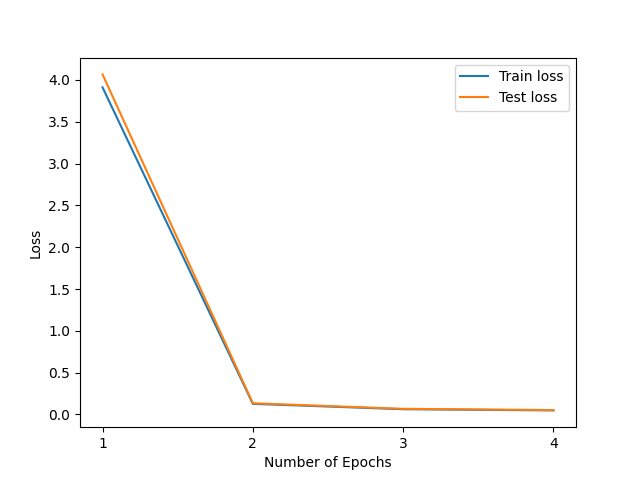
\includegraphics[width=0.85\linewidth]{correct_train_test_loss2piece.png}
    \caption{Train and test loss for the neural net to predict 2 cuts with one hidden layer consisting of 128 neurons.}
    \label{fig:train_test_2pieces}
\end{figure}

As it can be seen in figure \ref{fig:train_test_2pieces}, the performance on the training and test dataset is almost identical, meaning the model performs almost perfectly on the test set.\\
One reason for this behavior is probably due to the artificial nature of the data.
Since it performs so well on the unseen test set, I assume also good performance on completly new data.\\
After that, I trained the model on 8563 training tuples that created beforehand.
I wanted to compare the solution times for different hyperparameter combinations, so I trained multiple models.
These models were then benchmarked on samples from the test set to compare the respective computation times.

For all combinations I only used models with one hidden layer, since one was already sufficient to create good predictions and more would probably just overfit the data.
I tried multiple quantities of hidden neurons, aside from the proposed 128, and up to 110 hidden neurons the trained models were never able to solve every presented problem instance, meaning that the predicted optimality cuts lead to infeasibility or cycling of the solver.
Because of that, I only looked at models with 128 hidden neurons. \\
The hyperparameter left to vary was the number of cutting planes that the neural network predicts.
As the representation of the problem instance is 5-dimensional, it is not expected that the network is able to reliably predict more than two cuts, since each cut consists of two coefficients, if the decision variable is one-dimensional, so for two cuts four coefficients are needed. \\
This implies that the model should only be able to predict two optimality cuts.
Of course, this is only the case if the coefficients are independent of each other, which is probably does not hold.
Because of that, I also chose to look at the results for three predicted cuts.

For each hyperparameter, the training and test data had to be trimmed in order to provide uniform output dimensions, since the neural network can not deal with a variable number of output dimensions.
This lead to an effective reduction of the dataset size by about 10 to 20 samples. 
For each hyperparameter configuration, the respective model was trained and used to predict optimality cuts on five randomly selected instances from the test set.
These instance were solved by using the standard SDDP algorithm and the $v$-SDDP algorithm.
The comparison of the respective solution times is visualized in figure \ref{fig:Solution Comparison}.
\begin{figure}[h]
    \centering
    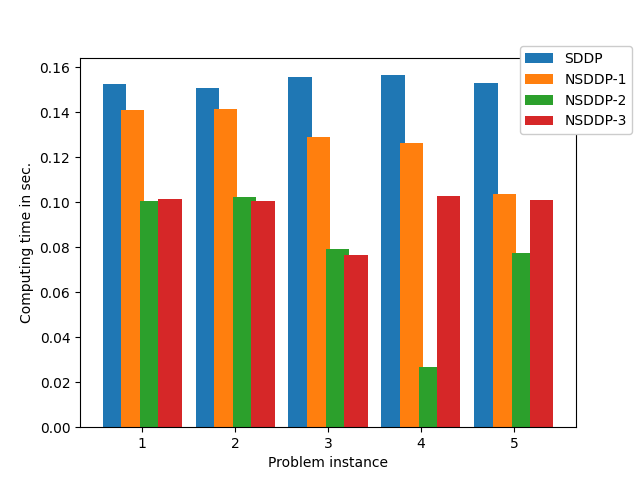
\includegraphics[width=\linewidth]{Computing_comparison_128hidden_neurons.png}
    \caption{Comparison of computing time on five random problem instances from the test data set. SDDP describes the solution time of the standard SDDP algorithm. NSDDP-1 describes the computing time of $v$-SDDP with one predicted cutting plane}
    \label{fig:Solution Comparison}
\end{figure}

It is clear from figure \ref{fig:Solution Comparison} that more predicted optimality cuts provide better computation times.
An interesting comparison is between the computation time of $v$-SDDP with two and three optimality cuts, respectively. \\
In general, it would seem that the more cutting planes are predicted, the lower the computation time.
However, as seen in problem instance four and five, the model with just two cutting planes is substantially faster than the one with three cutting planes. \\
Since the solution with two cutting planes in instance four is computed almost instantly, it can be assumed that the cutting planes provided from $v$-SDDP in this instance are all the cutting planes that are needed to compute an optimal solution.
The three generated cutting planes possess less predictive power, as they have a longer computing time. \\
This could be the result of my argument that in my specific use case only the prediction of two optimality cuts should be applicable, since three cuts are too high-dimensional to reliable make predictions with this kind of network.
It seems that for some instances the approach with three cuts is able to achieve slightly better performance but is not able to generalize that on all instances.

It could be shown that the NSDDP approach can lead to an acceleration of the computing time of $30-40\%$ on average using more than one cutting plane.
However, the used two-stage news-vendor problem instances are very small problem and the neural network still needed 128 neurons in the hidden layer, which indicates that this approach needs a lot of resources.

\section{Discussion and Conclusion}\label{Discussion and conlcusion}
In this section the results from my experiments are discussed and an outlook to possible further research topics is given based on my observations.
Finally, the seminar paper and its insights will be summarized.
\subsection{Discussion}\label{Discussion}
As the previous sections showed, the NSDDP is a valid approach to improve computation time for stochastic programs.
While the approach of using structures like neural networks to compute value function approximations is not particularly new, similar approaches for value function approximation where already presented in 1999 in \cite{Neuro-dynamic-programming}, the approach of using a meta machine learning approach that incorporates information about the problem structure is novel.
A further novel addition is the use of the earth-movers distance in the loss function instead of the usual squared, euclidean distance. \\
As shown in my experiments in section \ref{Own_computations}, the approach can lead to major speed-ups in the computation time. \\
The paper provided two methods to obtain faster computation times, the $v$-SDDP approach and the fast-inference SDDP approach. \\
The fast-inference SDDP approach was not further investigated in this seminar paper, however it is clear from the structure of this approach that it needs almost the same effort, if not more, than the NSDDP approach to set up, since it also required the training of a neural network and the additional training of a projection matrix $G$. \\
Furthermore, it is not clear how well the projection will generally work in practice.
The approach uses principal component analysis to calculate the projection matrix, however it can not be guaranteed that the point $x = G^Ty$ is feasible for the unprojected problem.

The major drawback from the NSDDP approach is that this method does not guarantee that a lower bound to the value function is computed.
That can lead, as seen in my experiments, to unsolvable problems that otherwise would be solvable.  \\
Furthermore, the approach stands and falls with the representation of the problem.
The smaller the representation of the problem, i.e. the fewer parameters are needed for the description, the more difficult it is to predict cutting planes reliably, as described in section \ref{Own_computations}.  \\
For example, if in a large problem description only one parameter varies, that however affects multiple constraints in a different way, either a complex representation of that behavior has to be defined or the NSDDP approach most likely cannot be applied, as the predictive power of just one parameter would be too small to predict multiple optimality cuts. \\
As seen in my experiments, the number of cuts was limited by the number of parameters and this constraint becomes harder to fulfill, the larger the space of the decision variables becomes and the smaller the representation of the problem instance is.
A disadvantage that exactly this approach wanted to solve.
With a look at practical applications, where decision variables are usually high-dimensional, this is a major downside of this approach. \\
Furthermore, the current approach requires that the representation of the problem instance is passed as a vector, which may not be able to transfer the information about structural dependencies of the specific problem instance.

Subsequent research could explore how, for example, convolutional neural networks could be used to extract structural information.
Convolutional neural network are mainly used in computer vision, as they learn a representation of pictures, which are just matrices with the respective color values as entries, also known as featuremaps \cite{ComputerVisionBook} which are then passed to a regular MLP.
This could possibly augment the NSDDP approach. \\
This could be especially interesting for problems were the problem structure allows for the application of decomposition techniques from the field of large-scale optimization, that would be overlooked in a vector representation.

Besides the aforementioned downsides, the NSDDP approach can lead to major computation time reductions that could be continuously improved, as more data naturally becomes available.
However, to exploit the new data, the model has to be retrained, which could take a long time and a lot of resources, depending on the model size. \\
Moreover, subsequent research could explore how well the fast-inference SDDP approach from \cite{NSDDP} works and if similar problems regarding infeasibility arise. \\
Furthermore, it could be researched how concepts like transfer learning could be incorporated into this approach so that this approach is not limited to the specific family of problems that it is trained on. \\
Especially looking at real world applications, where problem instances would be larger and the neural network more complicated, hence training and retraining the neural network would require a lot of resources, this could be used to reduce the resource requirements.

\subsection{Conclusion}\label{Conclusion}
This seminar paper presented an overview of the field stochastic optimization, what frameworks exist and what advantages and disadvantages each framework provides.
The current state-of-the-art algorithms were presented and the advantages and disadvantages were discussed. \\
The main disadvantage that was common for all but one approach, was the bad scalability for larger problems with more stages.
The stochastic dual dynamic programming algorithm was able to solve this shortcoming by sampling the scenario tree.
However, even this approach suffered from bad scalability as the number of necessary iteration for SDDP increased exponentially with the dimension of the decision variables. \\
The neural stochastic dual dynamic programming approach tries to solve these shortcomings by predicting optimality cuts based on a representation of the problem instance with a meta-machine learning model, which can be used as a warm start for the SDDP algorithm. \\
Furthermore, a projection to a low-dimensional representation of the problem can be provided, which can be solved faster and can be used to generate feasible points. \\
A potential application of NSDDP was presented with the unit commitment problem and the potential as well as the constraints of NSDDP for this particular application were highlighted. \\
Own Experiments were provided, which showcased that a speed-up of $30-40\%$ on average on the news-vendor problem can be achieved.
However, also the disadvantages were showcased, which were the reliability on the representation of the problem instance and that the NSDDP approach does not guarantee to create only lower bounds on the value function approximation. \\
In further research, it could be studied if approaches from computer vision are applicable to extract meaningful representations of the problem instances.

% \begin{thebibliography}{7}

% \bibitem{Nic10SW}
% \textsc{S. Nickel, O. Stein, K.-H. Waldmann,}
% \textit{Operations Research,}
% Springer, 2013.

% $\vdots$

% \end{thebibliography}
%\printbibliography
\medskip
\bibliographystyle{unsrt}
\bibliography{references}
\end{document}
